\section{Fahrspurregelung mittels modellprädiktiver Regelung}
In allen dynamischen Disziplienen des Carolo-Cups besteht die wichtige Teilaufgabe möglichst fehlerfrei einer in weiß auf schwarz aufgeklebten Fahrbahn zu folgen. Um diese Aufgabe zu erfüllen, wurde ein modellprädiktiver Regelansatz gewählt.\\ \\ 
Bei der modellprädiktiven Regelung (MPC) handelt es sich um eine Form der optimalen Regelung, bei der wiederholt eine Berechnung der optimalen Steuerung für ein System ausgehend von dessen aktuellem Zustand stattfindet. In vielen Bereichen finden MPCs immer häufiger Anwendung, da sie eine direkte Berücksichtigung von Beschränkungen erlauben und eine Form des strukturierten Reglerentwurfs ausgehend von der modellierten Systemdynamik darstellen. Dabei kann durch die geeignete Wahl der Kostenfunktion und deren Wichtungsparametern die Güte des Reglers geziehlt beeinflusst werden. Allerdings ergeben sich auch Schwierigkeiten bei der Verwendung von MPCs. Zum einen ist die Konvergenz der Optimierung gegen einen optimalen Wert für die Optimierungsvariablen und die Stabilität des geschlossenen Kreises insbesondere bei nichtlinearen Systemmodellen oft nur schwierig nachweisbar und zum anderen stellt das wiederholte Lösen des meist hochdimensionalen Optimierungsproblems während der Laufzeit in genügend schneller Geschwindigkeit eine große Herausforderung dar.
\\
\subsection{Problemformulierung für die modellprädiktive Regelung}
Im realen Anwendungsfall des oTToCAR-Projekts eignet sich eine Systemdarstellung in zeitdiskreter Form (\cite{ADA09}), bei der die Lösung des Optimierungsproblems weniger komplex ist und die ebenfalls zeitdiskreten Messwerte vom realen System weniger kompliziert integriert werden können. Demnach sind die diskretisierten Systemgleichungen wie folgt gegeben:
\begin{align*}
  \boldsymbol{x}(k+1)&=\boldsymbol{f}\left ( \boldsymbol{x}(k), \boldsymbol{u}(k) \right )\\
  \boldsymbol{y}(k)&=\boldsymbol{g}\left ( \boldsymbol{x}(k) \right )\\
\end{align*}
mit den nichtlinearen Funktionen $\boldsymbol{f}\left ( \cdot \right )$ und $\boldsymbol{g}\left ( \cdot \right )$, wobei
\begin{align*}
  &\boldsymbol{x}(k) \in \mathcal{X}\subset\mathbb{R}^n\\
  &\boldsymbol{u}(k) \in \mathcal{U}\subset\mathbb{R}^m\\
  &\boldsymbol{y}(k) \in \mathcal{Y}\subset\mathbb{R}^r
\end{align*}
Ausgehend vom aktuellen Zustand $\boldsymbol{x}(k)$ des zu regelnden Systems, der wenn nicht messbar geschätzt werden muss, wird anhand des Systemmodells das zukünftige Systemverhalten
\begin{align*}
  \boldsymbol{x_p}=\left\{ \boldsymbol{x}(k+1),\dots,\boldsymbol{x}(k+n_p)\right\}
\end{align*}
bis zum Prädiktionshorizont $n_p$ unter der Optimierung einer Sequenz von Eingängen
\begin{align*}
  \boldsymbol{u}=\left\{ \boldsymbol{u}(k),\dots,\boldsymbol{u}(k+n_c-1)\right\}
\end{align*}
bis zum Stellhorizont $n_c$ vorhergesagt. Aus der gefundenen optimalen Eingangssequenz $\boldsymbol{u}^*$ wird der erste Eintrag $\boldsymbol{u}^*(k)$ auf das zu regelnde System angewandt. Im nächsten Zeitschritt kann der neue Zustand gemessen bzw. geschätzt werden und die Optimierung beginnt von neuem. Ziel dabei ist es einer Referenztrajektorie $\boldsymbol{x_r}$ zu folgen.\\ \\
Für das an jedem Zeitschritt $k$ zu lösende Minimierungsproblem wurde die benötigte Kostenfunktion $J$ in quadratische Form mit $\boldsymbol{x_p}$ und $\boldsymbol{u}$ als Optimierungsvariablen aufgestellt:
\begin{align*}
	\underset{\boldsymbol{x_p, u}}{\text{min}}\;&J:=\sum_{i=k+1}^{k+n_p} \left [\boldsymbol{x}_{p}(i)-\boldsymbol{x}_{r}(i)\right ]^T\boldsymbol{Q}_i\left [\boldsymbol{x}_{p}(i)-\boldsymbol{x}_{r}(i)\right ] +\sum_{j=k}^{k+n_c-1} \boldsymbol{u}^T(j)\boldsymbol{R}_j\boldsymbol{u}(j)\\
	s.t.\;&\boldsymbol{x_p}(i+1)=\boldsymbol{f}\left ( \boldsymbol{x_p}(i), \boldsymbol{u}(i) \right ),\quad i=k,...,k+n_c-1\\
	&\boldsymbol{x_p}(i+1)=\boldsymbol{f}\left ( \boldsymbol{x_p}(i), \boldsymbol{u}(k+n_c-1) \right ),\quad i=k+n_c,...,k+n_p-1
\end{align*}
Mit den Vektoren
\begin{align*}
	\boldsymbol{x}_p(k)&=\left [ \boldsymbol{x}_p(k+1\mid k),\dots,\boldsymbol{x}_p(k+n_p\mid k) \right ]^T\\
	\boldsymbol{x}_r(k)&=\left [ \boldsymbol{x}_r(k+1),\dots,\boldsymbol{x}_r(k+n_p) \right ]^T\\
	\boldsymbol{u}(k)&=\left [ \boldsymbol{u}(k),\dots,\boldsymbol{u}(k+n_c-1) \right ]^T
\end{align*}
und den dazugehörigen positiv definiten Wichtungsmatrizen $\boldsymbol{Q}_i\in\mathbb{R}^{n\times n}\;(i=1, ...,n_p)$ und $\boldsymbol{R}_j\in\mathbb{R}^{m\times m}\;(j=0, ...,n_c-1)$. Weiterhin lässt sich das Optimierungsproblem um einfache Beschränkungen der Eingänge
\begin{align*}
  \boldsymbol{u}_{min} \leq \boldsymbol{u}(i) \leq \boldsymbol{u}_{max},\quad i=k,...,k+n_c-1
\end{align*}
und Zustandsbeschränkungen der Form
\begin{align*}
  \boldsymbol{A}\boldsymbol{x}_p(i) \leq \boldsymbol{b}\quad i=k+1,...,k+n_p
\end{align*}
erweitern.

\subsection{Konkrete Implementierung der Fahrspurregelung für das oTToCAR}
Die konkrete Implementierung der Fahrspurregelung auf der Recheneinheit des oTToCARs macht weitere Vorarbeit, wie das erstellen der Referenztrajektorie und Anpassungen des allgemeinen Ansatzes für die MPC wie gewisse Vereinfachungen, um die Regelung mit einer Rate von 50Hz betreiben zu können, nötig.
\subsubsection{Dimension der Optimierungsvariable}
Als Systemeingänge für das Fahrzeugmodell sind der Lenkeinschlag der Räder $u_1=\delta$ und das Motordrehmoment $u_2=M_A$ vorhanden, demnach ergibt sich der Stellgrößenvektor zum Zeitpunkt $k$ zu $\boldsymbol{u}(k)=[u_1(k), u_2(k)]^T$. Da sich die prädizierten Zustände $\boldsymbol{x}_p$ aus den Gleichungsnebenbedingungen berechnen lassen, ergibt sich die Dimension der Optimierungsvariable also zu $2\cdot n_c$.
Je größer man $n_c$ wählt, desto besser lässt sich z.B. die Geschwindigkeit in Abhängigkeit zur Entfernung und Krümmung einer bevorstehenden Kurve begrenzen oder Schwierigkeiten beim Durchfahren von S-Kurven bewältigen. Allerdings nimmt dadurch auch die Dimension der Optimierungsvariable zu, was dazu führt, dass die Grenzen der verfügbaren Rechenzeit zum Lösen des Optimierungsproblems während der Laufzeit schnell erreicht werden.
\subsubsection{Referenztrajektorie}
Mit einer auf dem Fahrzeug befestigten Kamera lässt sich die zu verfolgende Fahrbahn wahrnehmen. Diese Wahrnehmung liefert mit einer Rate von bis zu 50Hz eine Polylinie der erkannten Fahrbahnmarkierung projiziert auf die rechte Fahrspur. Diese Polyline kann je nach erkannter Fahrbahn aus einer unterschiedlich Anzahl von Punkten mit variablem Abstand zu einander bestehen.\\ \\
Um diese Polylinien als Referenztrajektorie für die MPC nutzen zu können, werden zu kurze Polylinien zunächst soweit extrapoliert, dass ein Vergleich zwischen Prädiktion zum Zeitschritt $k+np$ und Referenz in jedem Fall möglich ist. Anschließend werden die Koordinaten der Punkte auf der Polylinie als Funkion in Abhängigkeit der summierten Wegstrecke zwischen den Punkten (vom Auto ausgehend) hinterlegt, um diese als Referenztrajektorie zu den dazugehörigen Werten aus der Prädiktion mit der zurückgelegten Wegstrecke $s_i = iv\Delta t$ interpolieren zu können. Dabei ist $v$ die Geschwindigkeit der Fahrzeuges. In Abb. \ref{fig:referenz} ist ein Beispiel einer Referenztrajektorie dargestellt.
\begin{figure}[t]
\centering
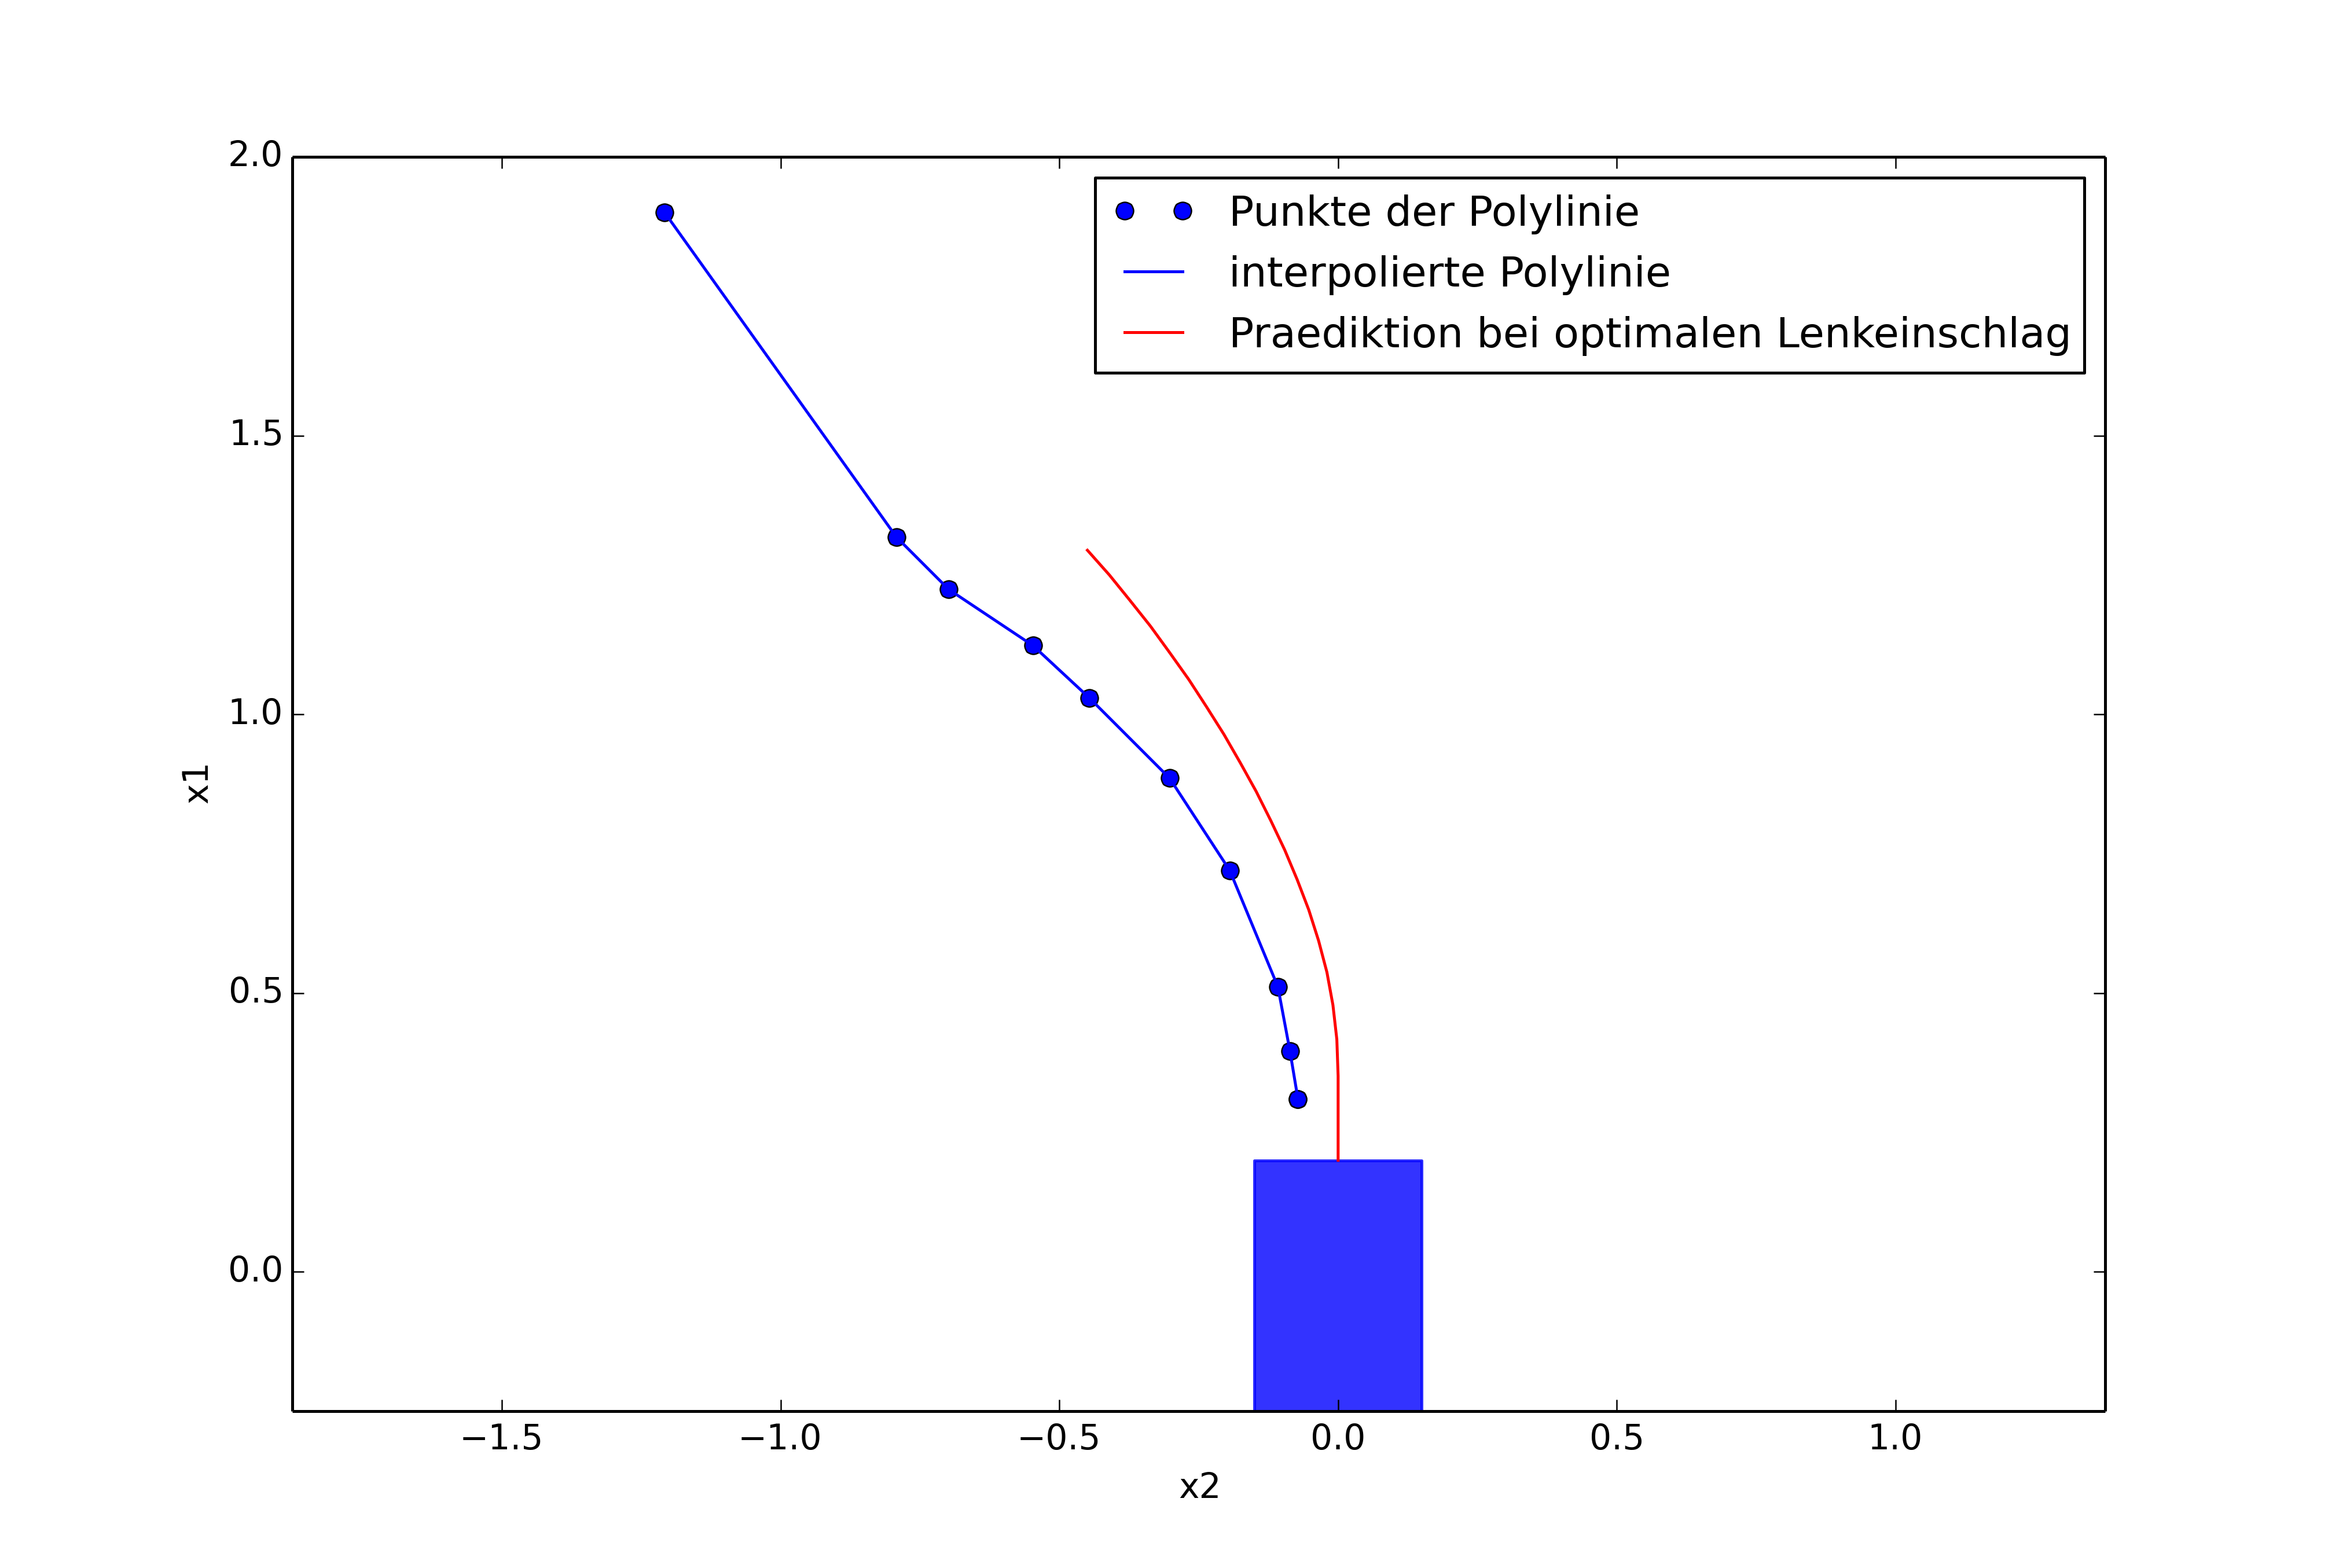
\includegraphics[scale=0.53]{Bilder/Reference.png}
\caption{Veranschaulichung der Referenztrajektorie und des prädizierten Verhaltens aufgetragen im Weltkoordinatensystem $x_1$ über $x_2$ in Meter}
\label{fig:referenz}
\end{figure}
Die Terme $\left [\boldsymbol{x}_{p}(i)-\boldsymbol{x}_{r}(i)\right ]$ in der Kostenfunktion werden demnach durch $\left [\boldsymbol{x}_{p}(i)-\boldsymbol{x}_{r}(s_i)\right ]$ ersetzt.\\ \\
Das Modell liefert als $x_1$ und $x_2$ die globale Position des Autos und den dazugehörigen Gierwinkel $x_3=\psi$. Da bisher noch keine globale Karte implementiert ist, wird jedes Mal, wenn eine neue Polylinie übermittelt wird die jeweils lokal gültige Weltkarte auf das Fahrzeugkoordinatensystem zurück gesetzt (Fahrzeugposition und Gierwinkel werden auf 0 zurück setzen.) Es ist kurzzeitig möglich, bei Ausbleiben einer verlässlichen neuen Polylinie, weiter an der letzten Referenztrajektorie weiter zu fahren, in dem man den Zustand bezogen auf das letzte lokal gültige Weltkoordinatensystem mit Hilfe des Modells schätzt. Dies ist allerdings nur für sehr kurze Zeiten (einzelne ausbleibende Polylinien) verlässlich.
\subsubsection{Vereinfachungen}
Aufgrund zwischenzeitlich erschöpften Rechenkapazitäten auf dem Fahrzeug während der Entwicklungsphase wurde der modellprädiktive Ansatz zunächst auf die einfachste denkbare Implementierung vereinfacht. Dabei wurde darauf verzichtet die Motorsteuergröße mit zu optimieren und der Stellhorizont für den Lenkeinschlag ist auf $n_c=1$ begrenzt. Aufgrund trotzdem zufriedenstellender Ergebnisse wurde an dieser Vereinfachung auch im Carolo-Cup festgehalten.\\ \\
Im nun eindimensionalen Optimierungsproblem lässt sich der Verlauf der Kostenfunktion in Abhängigkeit vom Lenkeinschlag sehr anschaulich darstellen. Schnell wird dabei klar, dass die Kostenfunktion im Bereich der real möglichen Lenkeinschläge eine Parabelform aufweist. Die Scheitelpunkt der approximierten Variablen zu berechnen. genau genug.\\
Kostenfunktion wie Parabel im Bereich unseres Interesses, an kann mit 3 Funktionsaufrufen den Schritt bestimmen, der zum Approximierten Optimum führt. Durch genügend hohe Wiederholrate ist das Ergebnis genau genug.\\ \\
Die Vorgabe der Geschwindigkeit erfolgt dabei aus einer einfachen Abhängigkeit von der mittleren prädizierten Gierrate. 
Skalierbarkeit\\
Scheitelpunkt -> Newtonschritt der quadratischen Kostenfunktion\\

Lösen der Modellgleichungen mit konstanter geringer Geschwindigkeit, da für hohe Geschwindigkeiten noch keine passenden Modellparameter bestimmt werden konnten.
\subsubsection{Stabilität}
Um Sicher zu gehen, dass der Algorithmus immer gegen ein Optimum konvergiert wurde die in implementierten Fall skalare Kostenfunktionen in der Parcour fahrt in möglichst vielen denkbaren Positionen aufgenommen und überprüft, dass sich kein Fall ergibt, in dem das Optimierungsproblem in relevanten Bereich nicht convex ist. ob sich Fälle ergeben in denen die Kostenfunktion im relevanten Bereich der möglichen Lenkeinschläge nicht convex ist. Abb. \ref{fig:parabel} zeigt das Ergebnis dieser Untersuchung. Es ist zu erkennen, dass die Kostenfunktion nur in wenigen Ausnahmefällen einer nach unten geöffneten Parabel ähnelt. Der hierbei berechnete Lenkeinschlag wird nicht auf das System gegeben, stattdessen wird mit dem vorherig berechneten Lenkeinschlag weiter gefahren und auf die nächste Polylinie von der Wahrnehmung gewartet. [[[[Bzw. an der alten Polylinie weiter gefahren]]]] Dank der relativ hohen Wiederholrate des Reglers stellen diese vereinzelten Ausfälle kein Problem dar.
\begin{figure}[t]
\centering
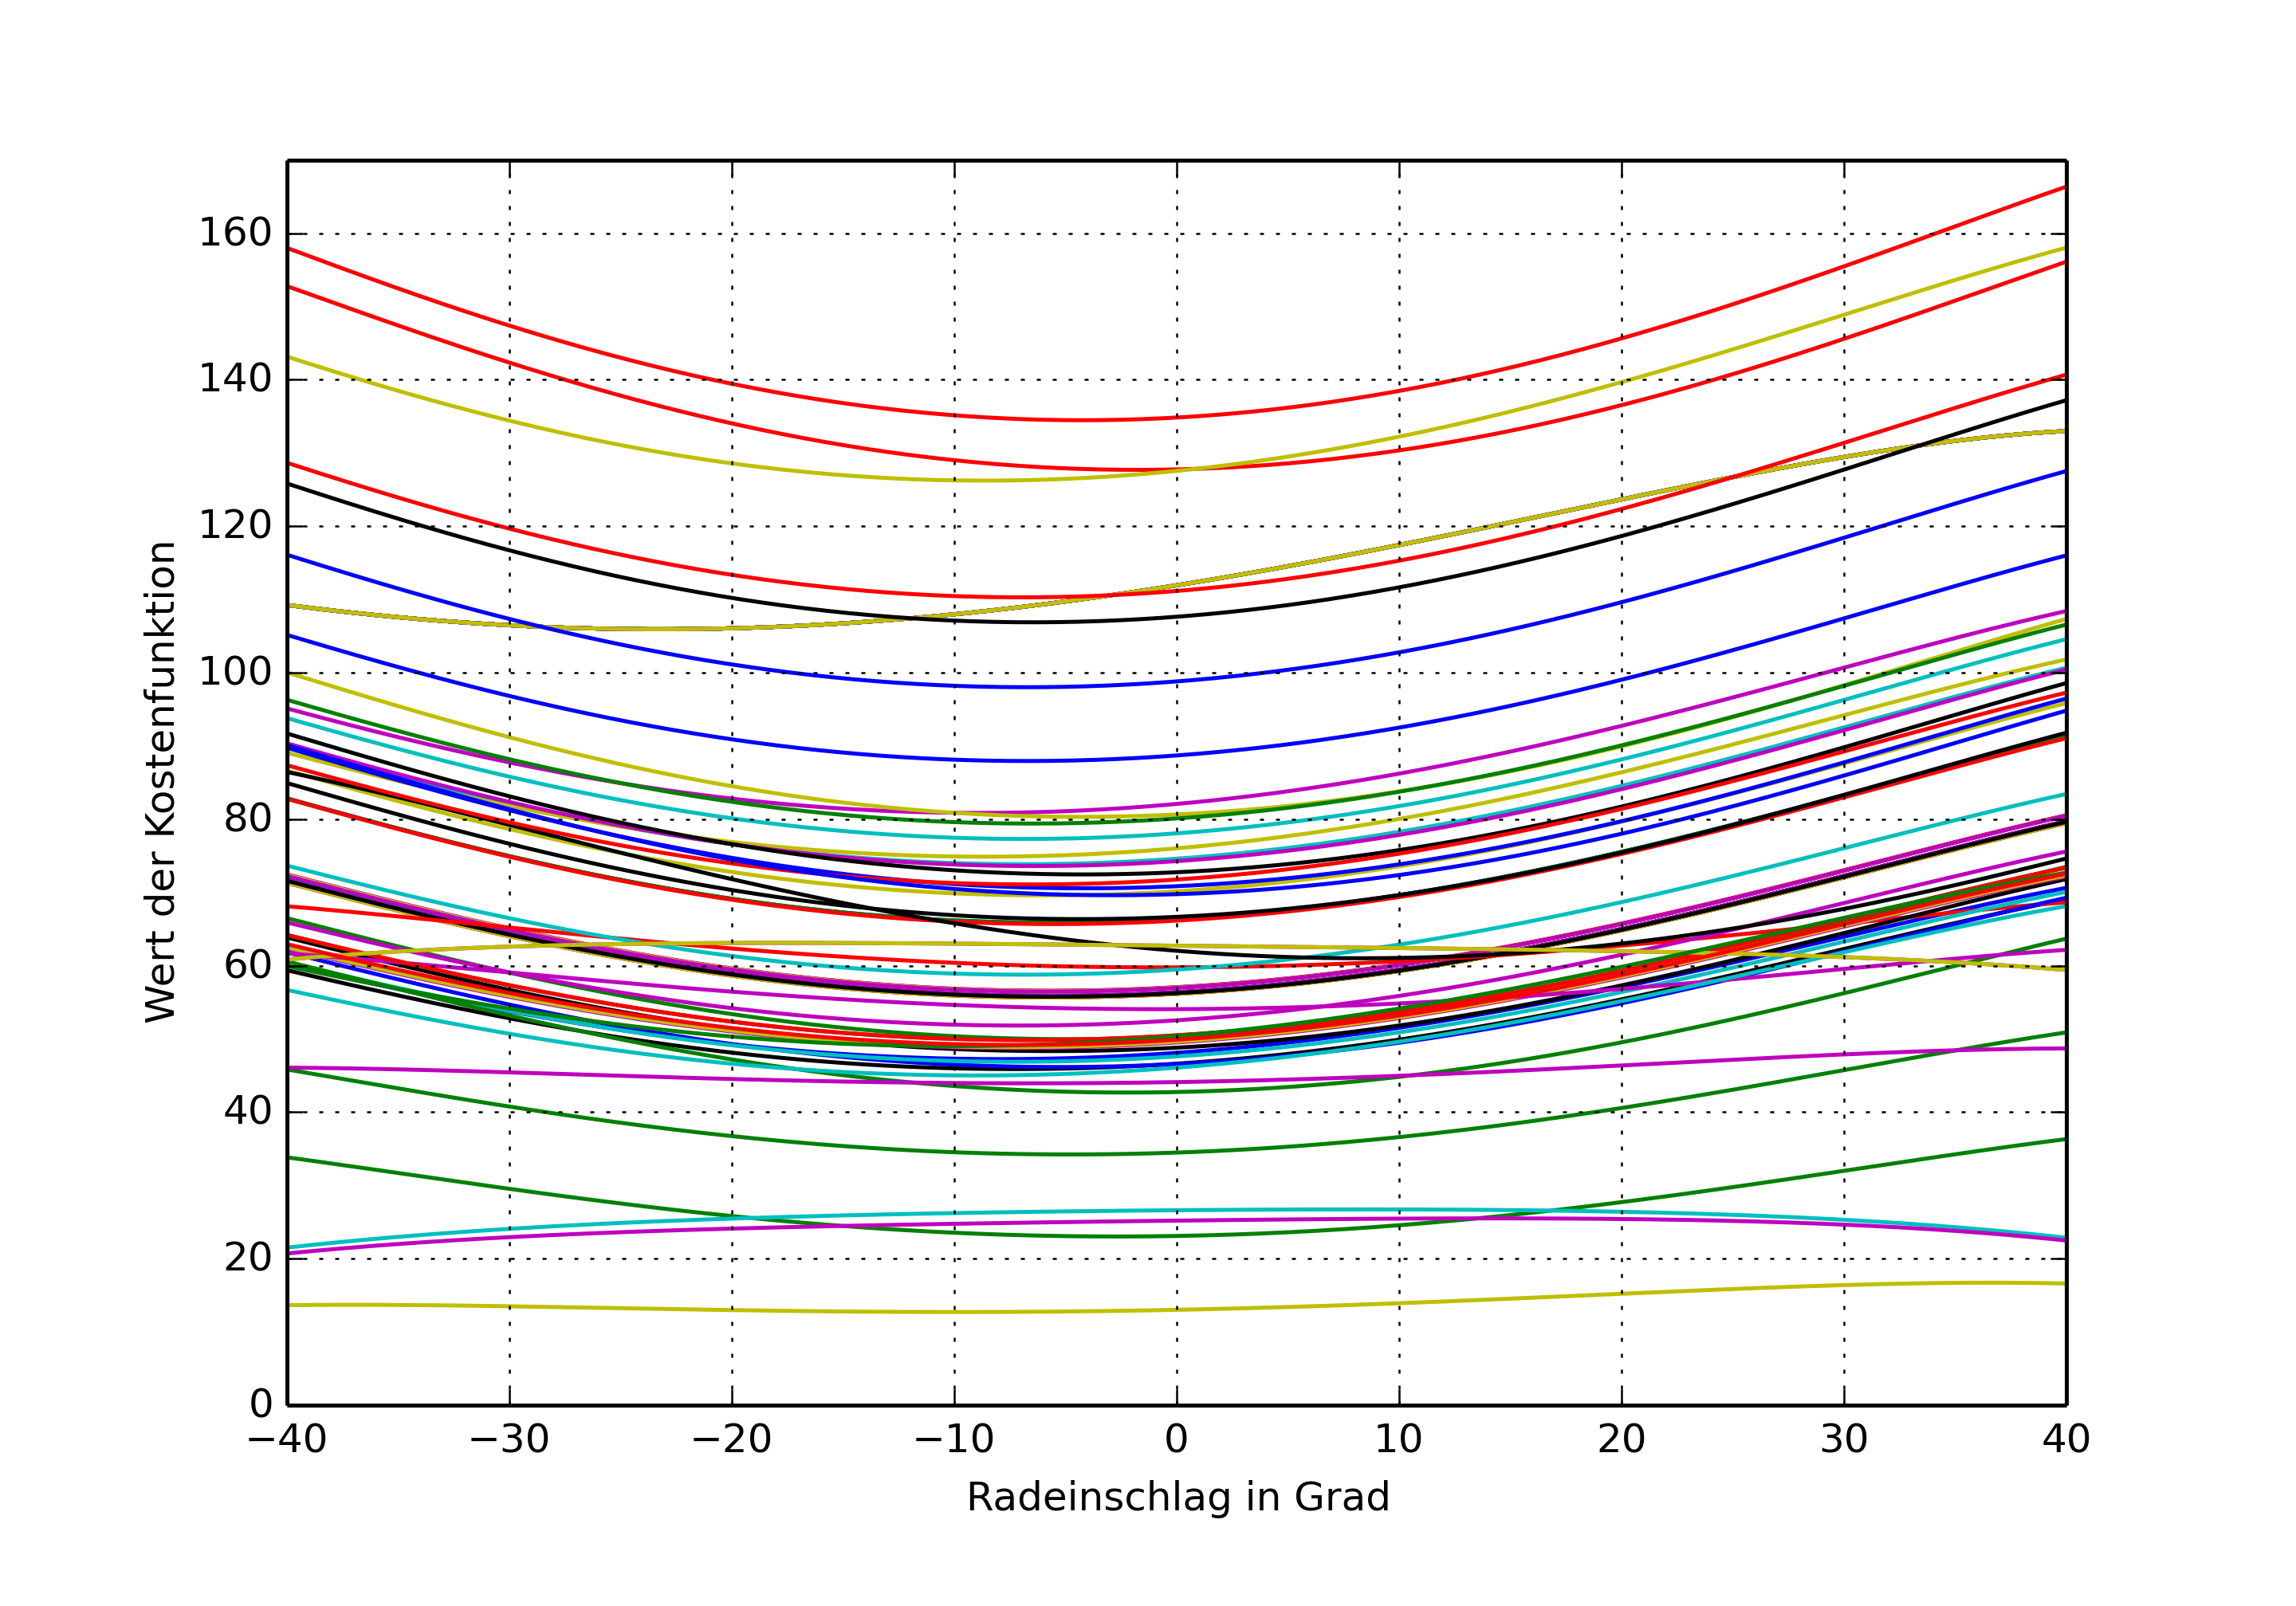
\includegraphics[scale=0.75]{Bilder/Parabeln.png}
\caption{Kostenfunktion in Abhängigkeit vom Radeinschlag in verschiedenen Fahrzeugpositionen}
\label{fig:parabel}
\end{figure}

\subsubsection{Beschränkungen}
Hinzufügen von ~
\subsection{Spurwechsel}
\begin{wrapfigure}{r}{8cm} 
%\begin{figure}[t]
\centering
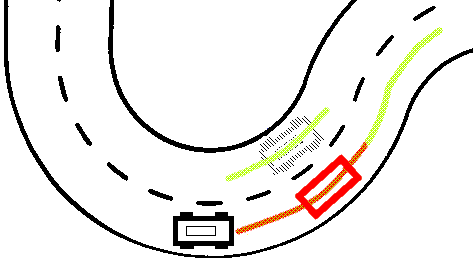
\includegraphics[scale=0.55]{Bilder/Spurwechsel.png}
\caption{Verschieben der Referenztrajektorie auf die linke Fahrspur bei erkanntem Hindernis}
\label{fig:spurwechsel}
%\end{figure}
\end{wrapfigure}
Polylinie um Fahrspurbreite verschieben, wenn Hindernis erkannt, wie in Abb. \ref{fig:spurwechsel} dargestellt. MPC findet optimale Trajektorie zu den verschobenen Punkten. Ein Problem stellt dabei allerdings die Wahrnehmung dar, weil bei starken Einlenken die Fahrbahn aus dem Sichtfeld der Kamera verschwindet. Alternativ eine Trajektorie vorzugeben bei der die Fahrbahn weiterhin wahrgenommen wird, ist nicht denkbar, da Hindernisse nach einer Kurve oft erst spät erkannt werden und deshalb Spurwechsel auf möglichst kürzester Distanz nötig sind. Da das Verfolgen der zuletzt gesehenen Polylinie wegen Modellungenauigkeiten und begrenzter Länge der Polylinie nur kurzzeitig ausreichend gut funktioniert, schlägt diese Strategie immernoch häufig fehl. Dazu wird allerdings eine wirkliche globale Karte implementiert in der die komplette Referenztrajektorie eingetragen ist und die tatsächliche Position des Fahrzeugs im Weltkoordinatensystem anhand der erkannten Strecke besser geschätzt werden kann.

\subsection{Dynamic Reconfigure}
In der Vorbereitung auf den Wettkampf hat sich herausgestellt, dass die kurzen Testzeiten auf der Originalstrecke gut ausgenutzt werden muss. Dazu musste vorher extrahiert werden, welche Parameter entscheidenen Einfluss auf die Güte haben. Diese konnten dann online während der Fahrt mit dem dynamic reconfigure Paket getuned werden. (Übersicht Parameter)\\
\subsection{Zukünftige Schritte}
Geschwindigkeit, Zusätzlich soll in der weiteren Entwicklung der Stellhorizont $n_c$ Erhöht werden um von der Prädiktion genauerer Information über die zukünftige Bewegung des Fahrzeuges zu bekommen. So wird erwaret dadurch schon eher vor Kurven bremsen und ebenfalls frühzeitiger aus Kurven heraus beschleunigen zu können, um eine Im Mittel höhere Geschwindikeit zu erreichen.\\ \\ Die Erstellung einer globalen Karte soll das Fahrverhalten außerdem robuster gegenüber Fehlwahrnehmungen der Fahrbahn machen und eine genauere Schätzung des aktuellen Zustands ermöglichen.